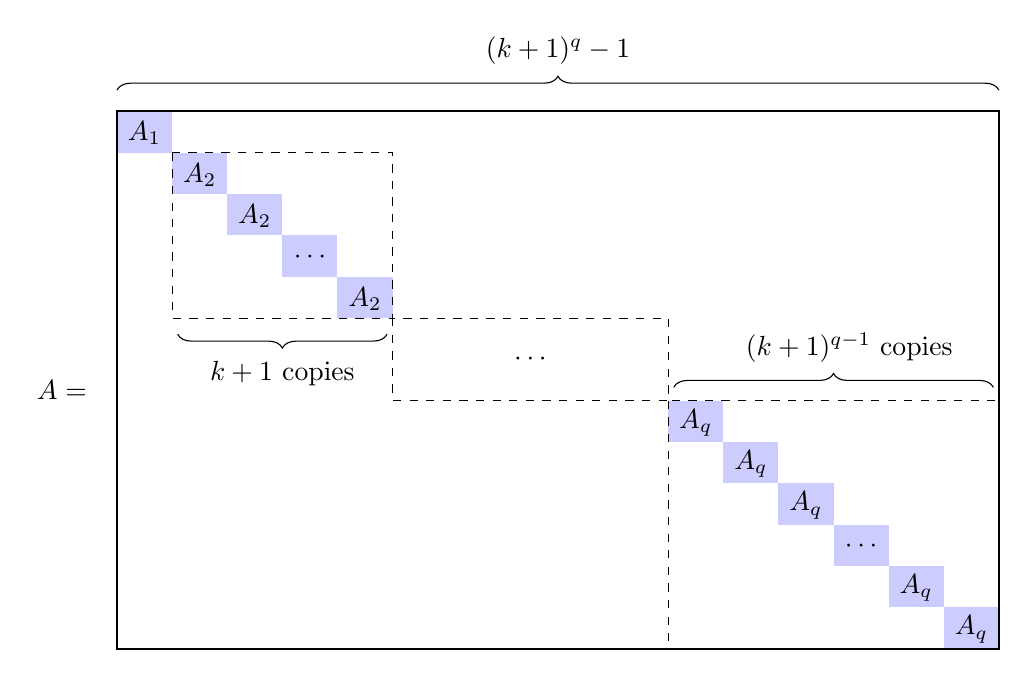
\begin{tikzpicture}[scale = 0.7]
	
%	\fill[blue!20] (0,4) rectangle (1,3);
%	\fill[blue!20] (1,3) rectangle (2,2);
%	\fill[blue!10] (2,2) rectangle (3,1);
%	\fill[blue!20] (3,1) rectangle (4,0);
%	
%	%	\draw[step = 1, black!20, thin] (0,0) grid (4,4);
%	\draw[thick] (0,0) rectangle (4,4);
%	
%	\node at (0.5, 3.5) {$\Psi_1$};
%	\node at (1.5, 2.5) {$\Psi_2$};
%	\node at (2.5, 1.6) {$\ddots$};
%	\node at (3.5, 0.5) {$\Psi_q$};
%	
	\node at (-1, -1.15) {$A =$};
	
%	\tikzset{shift={(6,0)}}
	
	
	%	\draw[step = 1, black!20, thin] (0,0) grid (4,4);
	
	\fill[blue!20] (0,3.90) rectangle (1,3.15);
	\node at (0.5, 3.5) {$A_1$};
	
	\fill[blue!20] (1,3.15) rectangle (2,2.40);
	\node at (1.5, 2.75) {$A_2$};
	\fill[blue!20] (2,2.40) rectangle (3,1.65);
	\node at (2.5, 2) {$A_2$};
	\fill[blue!20] (3,1.65) rectangle (4,0.90);
	\node at (3.5, 1.25) {$\cdots$};
	\fill[blue!20] (4,0.90) rectangle (5,0.15);
	\node at (4.5, 0.50) {$A_2$};

        \draw[dashed] (1,3.15) rectangle (5, 0.15);
	
	\draw [decorate,decoration={brace, amplitude=5pt, mirror, raise=1mm}]
	(1.1,0) -- (4.9,0) node[midway,yshift=-6mm]{$k+1$ copies};
	
	\draw[dashed] (5,0.15) rectangle (10,-1.35);
	\node at (7.5, -0.6) {$\cdots$};
	
	\fill[blue!20] (10,-1.35) rectangle (11,-2.10);
	\node at (10.5, -1.75) {$A_q$};
    
	\fill[blue!20] (11,-2.10) rectangle (12,-2.85);
	\node at (11.5, -2.50) {$A_q$};
    
	\fill[blue!20] (12,-2.85) rectangle (13,-3.60);
	\node at (12.5, -3.25) {$A_q$};
    
	\fill[blue!20] (13,-3.60) rectangle (14,-4.35);
	\node at (13.5, -4.00) {$\cdots$};
    
	\fill[blue!20] (14,-4.35) rectangle (15,-5.10);
	\node at (14.5, -4.75) {$A_q$};
    
	\fill[blue!20] (15,-5.10) rectangle (16,-5.85);
	\node at (15.5, -5.50) {$A_q$};
    
	\draw[dashed] (10,-1.35) rectangle (16,-5.85);
	
	\draw [decorate,decoration={brace, amplitude=5pt, raise=1mm}]
	(10.1,-1.25) -- (15.9,-1.25) node[midway,yshift=6mm,xshift=2mm]{$(k+1)^{q-1}$ copies};
	
	%\draw [decorate,decoration={brace, amplitude=5pt, mirror, raise=2mm}]
	%(20,0) -- (20,4) node[midway,xshift=7mm]{$qk$};
    
	\draw[thick] (0,3.9) rectangle (16,-5.85);
	
	\draw [decorate,decoration={brace, amplitude=5pt, raise=2mm}]
	(0,4) -- (16,4) node[midway,yshift=7mm]{$(k+1)^q-1$};
    
	
\end{tikzpicture}
